\documentclass{ctexbeamer}
\usetheme{CambridgeUS}
\usepackage[style=gb7714-2015ay]{biblatex}
\addbibresource{reference.bib}
\usepackage{graphicx}
\usepackage{float}
\usepackage{amsmath}
\usepackage{amssymb}
\usepackage{booktabs}
\setbeamertemplate{caption}[numbered]
\setbeamertemplate{bibliography item}{}
\setbeamertemplate{bibliography entry article}{}
\setbeamertemplate{bibliography entry title}{}
\setbeamertemplate{bibliography entry location}{}
\setbeamertemplate{bibliography entry note}{}
\title{基于KMV模型上市中小企业信贷风险研究}
\author{董晨阳}
\date{\today}
\begin{document}
\setbeamertemplate{bibliography item}{}
\setbeamertemplate{bibliography entry article}{}
\setbeamertemplate{bibliography entry title}{}
\setbeamertemplate{bibliography entry location}{}
\setbeamertemplate{bibliography entry note}{}
\AtBeginSection[]
{
    \begin{frame}{目录}
        \tableofcontents[sectionstyle=show/shaded,subsectionstyle=show/show/hide,subsubsectionstyle=show/hide/hide]
    \end{frame}
}
\maketitle
\begin{frame}{目录}
    \tableofcontents[hideallsubsections]
\end{frame}
\section{KMV模型理论}
\begin{frame}{引言}
    财务报表反映了公司的基本面信息,市场价格则反映了市场对公司未来的预期,因此基本面与市场面的双轮驱动框架更能准确度量信用风险。现代信用度量模型基于数理模型进行风险度量,拥有数理模型的精确性的特点,能够更加精准、客观地衡量企业信用状况。
    \begin{figure}
        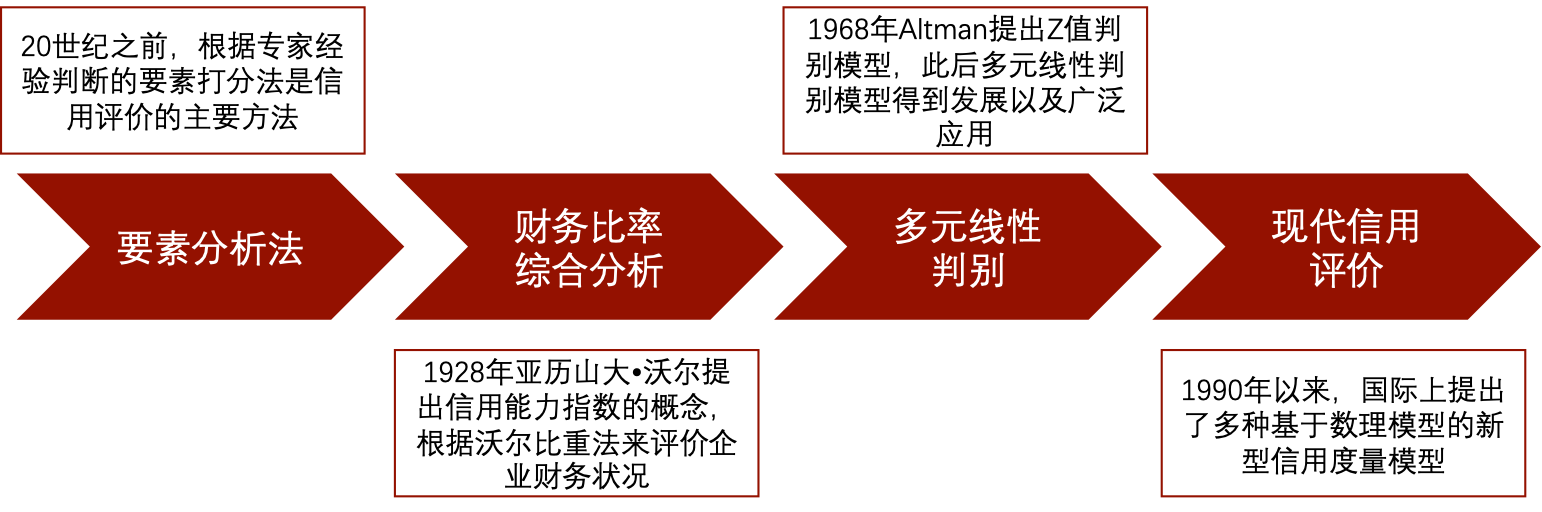
\includegraphics[width=0.8\linewidth]{fig/图片 1.png}
        \caption{信用风险度量方法发展历程}
    \end{figure}
\end{frame}
\begin{frame}{引言}
    \citet{彭伟2012基于}利用KMV模型研究我国2008-2011年的上市中小企业的信贷风险,对KMV模型参数进行了改进,用违约距离刻画中小企业信贷违约风险大小,发现违约距离具有一定的风险预测能力。

    在此研究基础上,\citet{彭伟2012我国上市中小企业信贷风险研究}将违约距离作为因子引入到更广泛的回归模型中,发现包含违约距离的回归模型对中小上市企业违约的判断准确性要高于不含违约距离的模型。
    \begin{figure}
        \begin{minipage}{0.48\linewidth}
            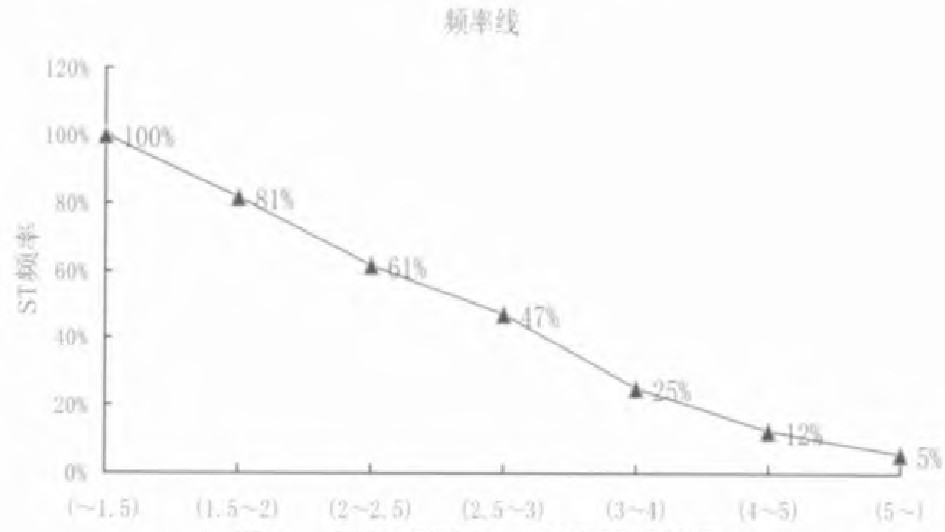
\includegraphics[width=\linewidth]{fig/1art.jpeg}
        \end{minipage}
        \begin{minipage}{0.48\linewidth}
            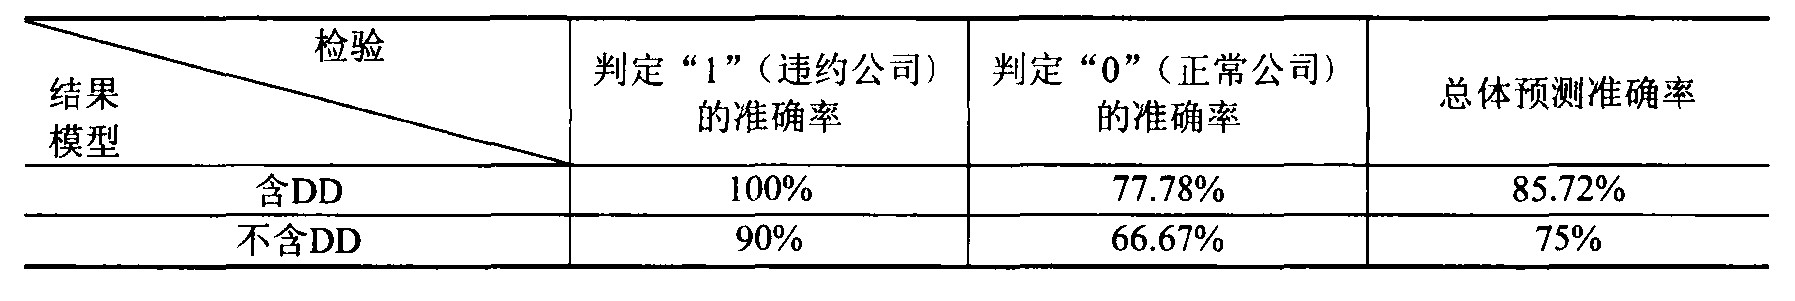
\includegraphics[width=\linewidth]{fig/2art.jpeg}
        \end{minipage}
        \caption{\citeauthor{彭伟2012基于}的主要结论}
    \end{figure}
\end{frame}
\subsection{KMV模型理论}
\begin{frame}{KMV模型的假设}
    KMV模型提出于1993年,KMV公司成立以来默默无闻,后一举成名于安然倒闭事件。在安然倒闭前约一年,大幅调高安然公司的违约概率,完败三大评级公司,后在2002年被穆迪收购。模型基于\citet{black1973pricing}和\citet{merton1974pricing}提出的BSM公式,假设包括
    \begin{itemize}
        \item 无交易成本与税收
        \item 相对静态的无风险收益率
        \item 无套利机会
        \item 企业的资产价值服从布朗运动
        \item 公司资产价值小于违约点则会选择违约
    \end{itemize}
\end{frame}
\begin{frame}
    \begin{center}
        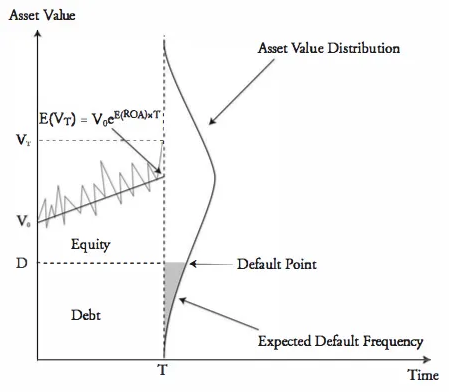
\includegraphics[width=0.6\linewidth]{img/KMV.png}
    \end{center}

    $V<DP$时企业将发生违约,观察需要多少个$V$标准差的变化使得公司价值落在违约点以下。
    \begin{equation*}
        DD=\frac{V_A-DP}{V_A\sigma_A}
    \end{equation*}
\end{frame}
\begin{frame}
    \begin{equation}
        DD=\frac{V_A-DP}{V_A\sigma_A}\label{eq:dd}
    \end{equation}
    逐项来看公式(\ref{eq:dd}):
    \begin{itemize}
        \item\only<1>{
        \textbf{资产价值$V_A$和波动率$\sigma_A$的计算}:将企业所有者权益视作欧式看涨期权,即\begin{equation*}
            E=\begin{cases}
                V_A-D & V_A>D    \\
                0     & V_A\le D
            \end{cases}
        \end{equation*}
        结合伊藤引理、企业股权价值本身服从几何布朗运动,可构造联立方程组得到\begin{eqnarray}
            E&=&V_AN(d_1)-e^{-rT}DN(d_2)\label{eq:ee}\\
            \sigma_E&=&\frac{V_A}{V_E} N(d_1)\sigma_A
        \end{eqnarray}其中$d_1=\frac{1}{\sigma_E\sqrt{T}}(\ln \frac{S}{L}+(\mu+\frac{1}{2}\sigma^2_E)T)$,$d_2=d_1-\sigma_E\sqrt{T}$

        所有者权益的价值和波动率都是公开的市场信息,从而可以计算得到$V_A$和$\sigma_A$
        }
        \only<2>{
            \textbf{$DP$的计算}:

            违约点 D 需要考虑了流动性的影响,给长短债赋予不同的权重,将短期债务和长期债务考虑进去。

            KMV公司的计算方式为加总所有的短期负债(即到期日小于 1 年的)的面值加上 50\%长期债务的面值。
        }
    \end{itemize}
\end{frame}
\begin{frame}
    \begin{eqnarray}
        DD&=&\frac{V_A-DP}{V_A\sigma_A}\\
        E&=&V_AN(d_1)-e^{-rT}DN(d_2)\\
        \sigma_E&=&\frac{V_A}{V_E} N(d_1)\sigma_A
    \end{eqnarray}
    如果资产价值服从对数正态分布,其连续增长率为$\mu$,公式(\ref{eq:dd})和(\ref{eq:ee})可以进一步化简为
    \begin{equation}
        DD=\frac{\ln \frac{V_A}{DPT}+(\mu-\frac{1}{2}\sigma^2)T}{\sigma_A\sqrt{T}}\label{eq:f}
    \end{equation}
\end{frame}
\begin{frame}
    得到违约距离$DD$后,KMV模型\textbf{基于历史违约数据库},依据违约距离可以映射出公司实际的期望违约频率。KMV 公司收集了包括3400上市公司和40000家非上市公司自1973年以来的资料,建立了庞大的数据库,得到从违约距离到预期违约率的映射关系,取得了良好的预测效果。
    \begin{figure}
        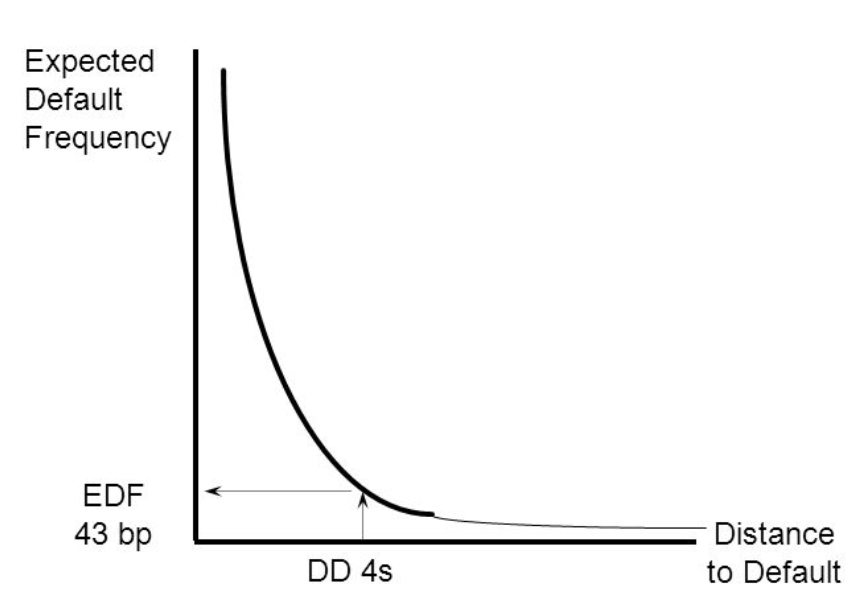
\includegraphics[width=0.5\linewidth]{fig/edf.png}
        \caption{根据历史 $DD\to EDF$映射}
    \end{figure}
\end{frame}
\subsection{KMV模型的价值}
\begin{frame}{KMV Pros}
    \begin{itemize}
        \item KMV模型运用了现代期权定价理论,建立违约预测模型,综合考虑了经验和模型,降低了主观因素对信用评估的影响,是对传统信用风险度量方法的一次重要革命。
        \item KMV 模型的信用风险衡量指标预期违约率主要来自股票市场价格变化的有关数据,可以及时反映信用风险水平的变化。该模型主要依赖股票市场数据和财务报表中的负债数据进行计算,能够降低会计信息失真对模型结果的影响。
        \item 股价中包含了投资者对于公司未来发展的预期,预期违约率中包含了投资者对信用状况未来发展趋势的判断,因此,该模型具有一定的前瞻性。
    \end{itemize}
\end{frame}
\begin{frame}{KMV Cons}
    \begin{itemize}
        \item 该模型假设公司的资产价值服从正态分布,但是事实上企业的资产价值经常会呈现出非正态的统计特征。
        \item 对上市公司而言,由于我国的股市有效程度较低,一方面许多上市公司的股价常常远超出公司的实际价值,另一方面企业资产价值特别是国有企业的资产价值并不能够完全反映到股票市值中,因而模型预测可能会被影响。
        \item 而对非上市公司而言,往往要借助一些会计信息或其他能够反映借款企业特征值的指标来替代模型中一些重要变量,同时还要通过对比分析最终得出该企业的期望违约概率,一定程度上就有可能降低计算的准确性。
        \item 模型不能区分不同类型的债务。不同类型债务之间由如偿还优先顺序、担保、契约等关系,KMV模型仅仅抽象出了短债和长债两个特征。
    \end{itemize}
\end{frame}
\section{实证与复现}
\subsection{数据预处理与描述性统计}
\begin{frame}
    \frametitle{“刚兑”神话时代何谓违约}
    我国信用债市场曾经维持着“刚兑”神话,公开市场债券违约首现于2014年的11超日债违约,早于\citet{彭伟2012基于}。截至目前(\today)债券违约仍以非上市公司为主。因此\citet{彭伟2012基于}选择以公司是否被“ST”为违约标志。
    \begin{figure}[H]
        \centering
        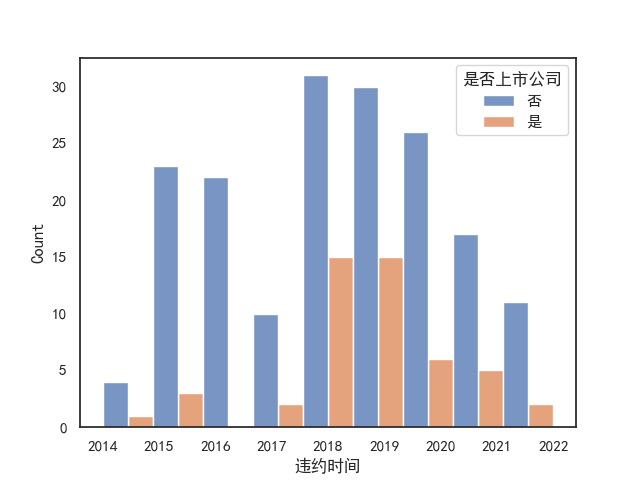
\includegraphics[width=0.6\linewidth]{img/发行人首次债券违约.png}
        \caption{迄今为止发行人首次债券违约时间分布}\label{fig:default}
    \end{figure}
\end{frame}
\begin{frame}
    \frametitle{“ST”戴帽视作信贷风险暴露}
    沪、深交易对财务状况异常的上市公司的股票交易进行特别处理Special Treatment,以表明具有较高的投资风险。实际情况中,虽然公司信贷违约与被 ST、*ST 不完全等同,但他们之间有较强的相关性,如超日债即为ST超日2011年发行的债券。时至今日我国信贷违约数据库尚在建设中,公开市场虽然打破了刚兑但数据量难以支撑大模型,这也是KMV模型应用的挑战之一。
    \begin{table}
        \centering
        \begin{tabular}{lcc}
            \toprule
            符号   & 经营连续亏损 & 预警           \\
            \midrule
            *ST  & 三年     & 退市预警         \\
            ST   & 二年     & 特别处理         \\
            S*ST & 三年     & 退市预警+还没有完成股改 \\
            SST  & 二年     & 特别处理+还没有完成股改 \\
            \bottomrule
        \end{tabular}
        \caption{沪深交易所对ST/*ST的规定}
    \end{table}
\end{frame}

\begin{frame}
    \frametitle{数据整理}
    清理数据后,共有89家满足\citet{彭伟2012基于}中小企业的定义(原文中有111家):
    \begin{enumerate}
        \item 2008 年 1 月 1 日之前在沪深证券交易所上市
        \item 流通股 ≤ 5 000 万股,且 2007 年 12 月31日前的主营收入或资产总额≤5 亿元。
        \item 删除那些停牌时间较长的公司,
        \item 没有 B 股、H 股股票
        \item 再进一步剔除掉股权波动率为0的样本点
    \end{enumerate}
\end{frame}

\begin{frame}
    \frametitle{数据描述性统计:股权部分}
    \begin{itemize}
        \item 波动率采用了GARCH(1,1)模型计算得出,
        \item 股权价值= 流通股市值 +(0.99576+0.60973$\times$每股净资产)$\times$非流通股数。
    \end{itemize}
    \begin{figure}
        \begin{minipage}{0.48\linewidth}
            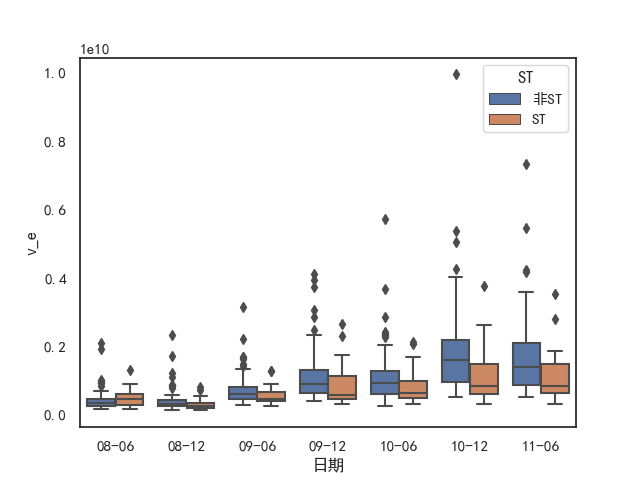
\includegraphics[width=\textwidth]{img/v_e.png}
        \end{minipage}
        \begin{minipage}{0.48\linewidth}
            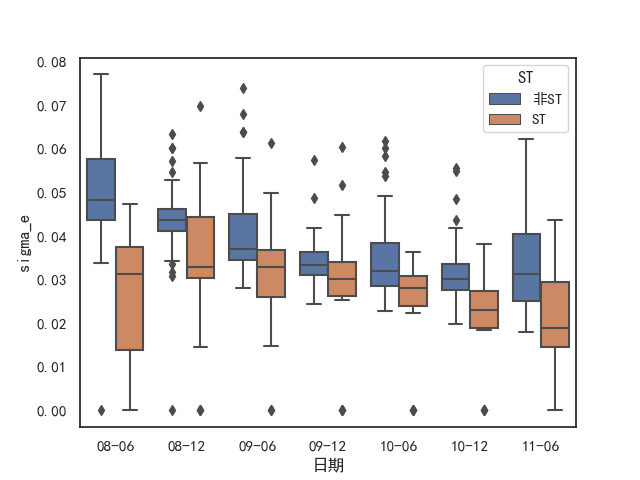
\includegraphics[width=\textwidth]{img/sigma_e.png}
        \end{minipage}
        \caption{股权价值(左)与波动率(右)}
    \end{figure}
\end{frame}
\begin{frame}
    \frametitle{数据描述性统计:债权部分}
    对所有08-11年的所有被实施ST的股票的总资产、短期负债和长期负债的价值进行了多元线性回归。大于KMV原始数据说明我国中小上市企业信贷风险相对国外更高,也可以说交易所判定是否ST较为严格。
    \only<1>{
        \begin{table}[H]
            \small\begin{center}
\begin{tabular}{lclc}
\toprule
\textbf{Dep. Variable:}    &       总资产        & \textbf{  R-squared:}      &     0.968   \\
\textbf{Model:}            &       OLS        & \textbf{  Adj. R-squared:} &     0.968   \\
\textbf{Method:}           &  Least Squares   & \textbf{  F-statistic:       }          &     4304.   \\
\textbf{Date:}             & Wed, 23 Nov 2022 & \textbf{  Prob (F-statistic):}          & 5.84e-211   \\
\textbf{Time:}             &     11:05:32     & \textbf{  Log-Likelihood:    }          &   -6294.1   \\
\textbf{No. Observations:} &         282      & \textbf{  AIC:               }          & 1.259e+04   \\
\textbf{Df Residuals:}     &         280      & \textbf{  BIC:               }          & 1.260e+04   \\
\textbf{Df Model:}         &           2      & \textbf{                     }          &             \\
\bottomrule
\end{tabular}
\begin{tabular}{lcccccc}
               & \textbf{coef} & \textbf{std err} & \textbf{t} & \textbf{P$> |$t$|$} & \textbf{[0.025} & \textbf{0.975]}  \\
\midrule
\textbf{流动负债}  &       1.3733  &        0.033     &    41.761  &         0.000        &        1.309    &        1.438     \\
\textbf{非流动负债} &       0.8951  &        0.053     &    16.821  &         0.000        &        0.790    &        1.000     \\
\bottomrule
\end{tabular}
\end{center}

            \caption{债权价值复现}\label{tab:1}
        \end{table}
    }
    \only<2>{
        \begin{figure}
            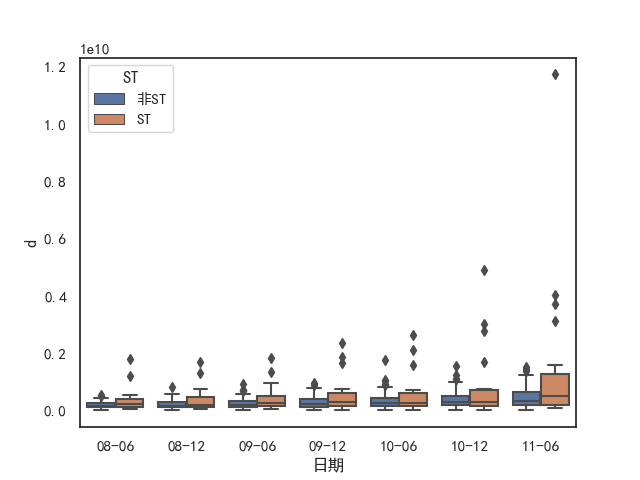
\includegraphics[width=0.6\linewidth]{img/d.png}
            \caption{违约点分布}
        \end{figure}
    }
\end{frame}

\begin{frame}
    \frametitle{数据描述性统计:其他}
    最后,作者将负债的平均期限假定为一年,企业预期资产价值增长的速度为公司资产净利率(作者提出的创新之一)。
    \begin{figure}[H]
        \centering
        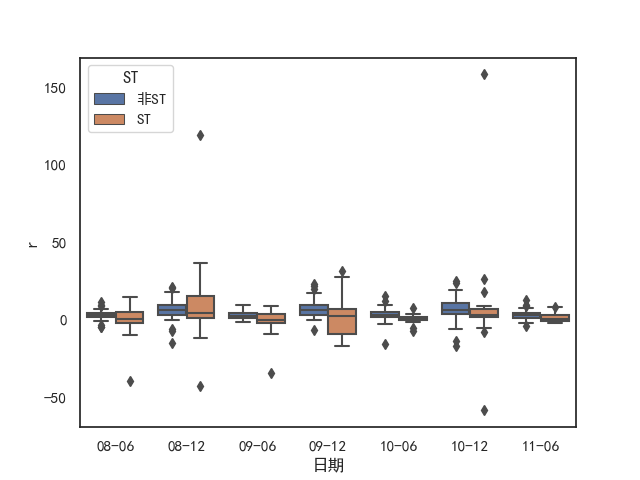
\includegraphics[width=0.6\textwidth]{img/r.png}
        \caption{公司资产净利率}
    \end{figure}
\end{frame}

\subsection{中小上市企业的违约距离}
\begin{frame}{违约距离计算}
    代入数据计算出整体不同年份的的违约距离如下图。由于彼时尚存在刚兑神话,难以通过违约距离$DD$得到相应的违约概率,因此作者停在这一步,用违约距离这一指标来衡量公司的信贷风险,并在之后的工作\cite{彭伟2012我国上市中小企业信贷风险研究}中进一步揭示有效性。
    \begin{figure}
        \begin{minipage}{0.48\linewidth}
            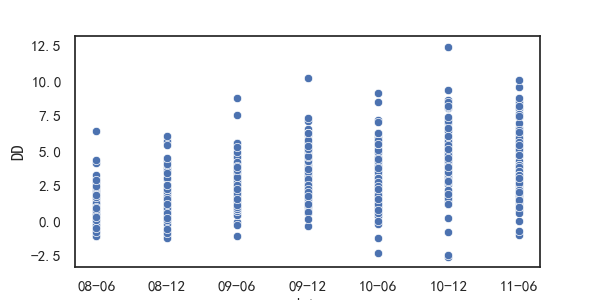
\includegraphics[width=\linewidth]{img/dd.png}
        \end{minipage}
        \begin{minipage}{0.48\linewidth}
            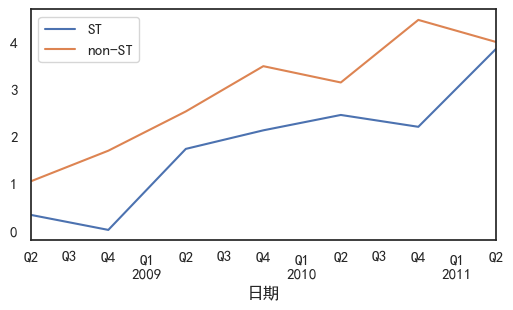
\includegraphics[width=\linewidth]{img/st-vs-non-st.png}
        \end{minipage}
        \caption{整体(左)、ST与非ST公司(右)的违约距离}
    \end{figure}
\end{frame}
\begin{frame}
    \frametitle{ ST与非ST公司违约距离是否差异显著}
    而对KMV模型是否有效,作者采用了两个独立样本的K-S检验和Mann-Whitney检验。K-S检验的显著性差异证明ST与非ST公司的违约距离不是同一个分布,MW检验显著性则验证了样本的均值并非相等。
    \begin{figure}[H]
        \begin{minipage}{0.48\linewidth}
            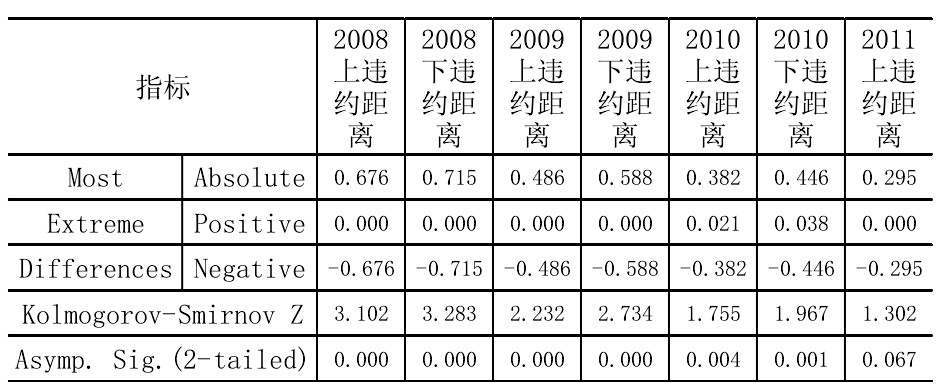
\includegraphics[width=\linewidth]{img/ks.jpeg}
        \end{minipage}
        \begin{minipage}{0.48\linewidth}
            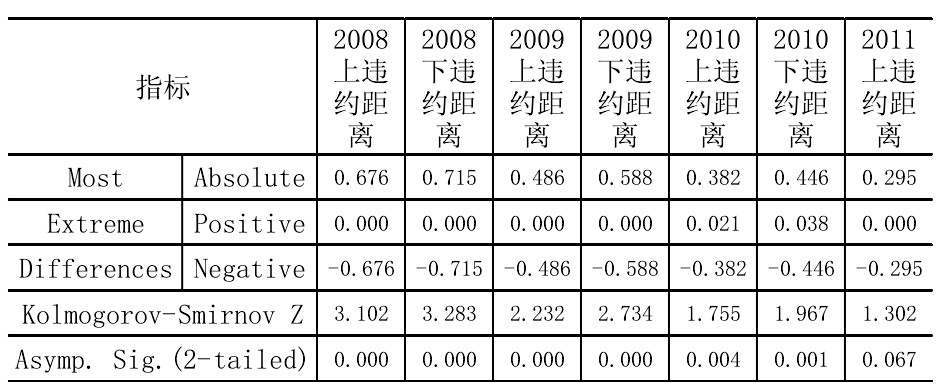
\includegraphics[width=\linewidth]{img/mw.jpeg}
        \end{minipage}
        \caption{原文中的KS(左)和MW(右)检验的结果}\label{fig:origin}
    \end{figure}
\end{frame}
\begin{frame}
    \frametitle{ ST与非ST公司违约距离是否差异显著}

    但复现结果显著性不强,可能由于样本数差异或数据处理方法差异,仅在部分年份显著,大部分时间表现显著性较弱。
    \begin{table}
        \tiny\begin{tabular}{lrrrrrrr}
\toprule
{} &  2008-06-30 &  2008-12-31 &  2009-06-30 &  2009-12-31 &  2010-06-30 &  2010-12-31 &  2011-06-30 \\
\midrule
statistic &    0.277778 &    0.222222 &    0.222222 &    0.194444 &    0.291667 &    0.291667 &    0.208333 \\
pvalue    &    0.236850 &    0.384915 &    0.384915 &    0.472853 &    0.206561 &    0.206561 &    0.427943 \\
\bottomrule
\end{tabular}

        \caption{复现的KS检验的结果}
    \end{table}
    \begin{table}
        \tiny\begin{tabular}{lrrrr}
    \toprule
    {}        & 2008-06-30 & 2008-12-31 & 2009-06-30 & 2009-12-31 \\
    statistic & 158.000000 & 47.000000  & 135.000000 & 78.000000  \\
    pvalue    & 0.230442   & 0.005167   & 0.284836   & 0.028662   \\
    \midrule
    {}        & 2010-06-30 & 2010-12-31 & 2011-06-30 &            \\
    statistic & 182.000000 & 131.000000 & 217.000000 &            \\
    pvalue    & 0.443427   & 0.091772   & 0.892414   &            \\
    \bottomrule
\end{tabular}

        \caption{复现的MW检验的结果}
    \end{table}
\end{frame}

\subsection{违约距离的影响因素}
\begin{frame}
    \frametitle{违约距离与总资产}

    公司规模理应是影响公司信用风险的重要因素。资产规模较大的公司一般而言具有更强的变现能力,因而其相应的违约距离也就更大。并且在实际的信贷市场中,大公司向银行争取贷款相对于中小企业而言显得更为容易,这也正是中小企业在信贷市场上“融资难、融资贵”,导致其信贷风险偏高的原因。
    \begin{table}[H]
        \centering
        \begin{tabular}{lrrrr}
    \toprule
    {}       & 2008-06-30 & 2008-12-31 & 2009-06-30 & 2009-12-31 \\
    pearsonr & -0.265334  & -0.221167  & -0.410335  & -0.230768  \\
    pvalue   & 0.016667   & 0.047233   & 0.000142   & 0.038201   \\
    \midrule
    {}       & 2010-06-30 & 2010-12-31 & 2011-06-30 &            \\
    pearsonr & -0.354095  & -0.444828  & -0.464128  &            \\
    pvalue   & 0.001182   & 0.000032   & 0.000013   &            \\
    \bottomrule
\end{tabular}

        \caption{违约距离与总资产的相关系数}\label{tab:asset}
    \end{table}
\end{frame}
\begin{frame}
    \frametitle{违约距离与股价波动率}
    股权市场上的波动率对KMV模型也有较大的影响,波动率越高违约距离越小。这可能是由于股权价值的高波动导致资产价值到预期违约距离的标准差倍数越小。
    \begin{table}[H]
        \centering
        \begin{tabular}{lrrrr}
\toprule
{} &  2008-06-30 &  2008-12-31 &  2009-06-30 &  2009-12-31  \\
pearsonr &   -0.023419 &   -0.312969 &   -0.254424 &   -0.184716\\
pvalue   &    0.835603 &    0.004444 &    0.021901 &    0.098770\\
\midrule
{} &  2010-06-30 &  2010-12-31 &  2011-06-30 &\\
pearsonr &  -0.249410 &   -0.121688 &   -0.327771& \\
pvalue   &   0.024741 &    0.279166 &    0.002817& \\
\bottomrule
\end{tabular}

        \caption{违约距离与股价波动率的相关系数}\label{tab:vol}
    \end{table}
\end{frame}
\begin{frame}
    \frametitle{违约距离与其他因素}
    但是,违约风险并非只与KMV模型相关。2008-2011是金融危机冲击后的时代,2008年时中小企业整体的违约距离更低,宏观层面与风险传染对信贷风险会有比较大的影响。或许由于写作时代的原因,作者并未涉及到宏观环境对公司信贷风险的影响。
    \begin{figure}
        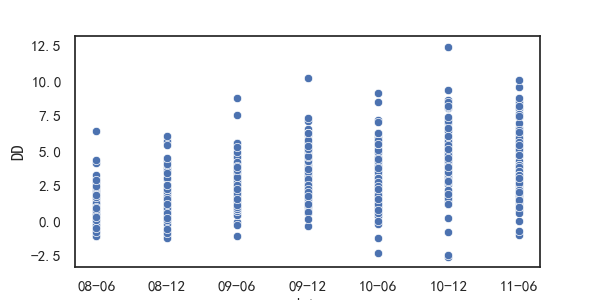
\includegraphics[width=0.8\linewidth]{img/dd.png}
        \caption{整体中小企业的违约距离}
    \end{figure}
\end{frame}

\subsection{违约距离对信贷风险的预测效果}
\begin{frame}
    \frametitle{文献中的样本错误}
    作者选择数据中2010-2011年间被ST的样本,研究其在被ST前的5个半年内违约距离DD值的变化规律,但数据选择有误
    \begin{columns}[c]
        \column{0.48\linewidth}
        \begin{figure}[H]
            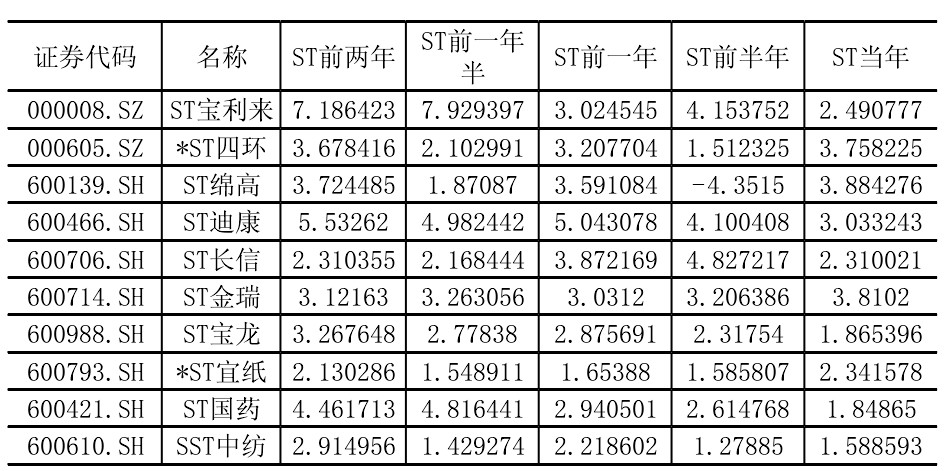
\includegraphics[width=\linewidth]{img/dd_origin.jpeg}
            \caption{原论文称这些公司为2010-2011年间被ST,但事实上均2008年便被ST}
        \end{figure}
        \column{0.48\linewidth}
        \begin{table}[H]
            \centering
            \tiny\begin{tabular}{lcc}
                \toprule
                       & ST天润     & *ST云投    \\
                \midrule
                ST前两年  & 0.238944 & 2.106469 \\
                ST前一年半 & 1.547428 & 4.392480 \\
                ST前一年  & 1.779768 & 3.959906 \\
                ST前半年  & 2.275831 & 2.631978 \\
                ST当年   & 1.222579 & 1.927210 \\
                \bottomrule
            \end{tabular}
            \caption{事实上的满足条件样本的违约距离}
        \end{table}
    \end{columns}
\end{frame}

\begin{frame}{违约距离对信贷风险的预测效果}
    复现结果在ST前一年半内表现较好,违约距离整体呈现走低的趋势。但是考虑到两年全量,表现差强人意。可能的解释是考虑两年时,金融危机的影响较大,因而导致整体的违约距离较低。
    \begin{figure}
        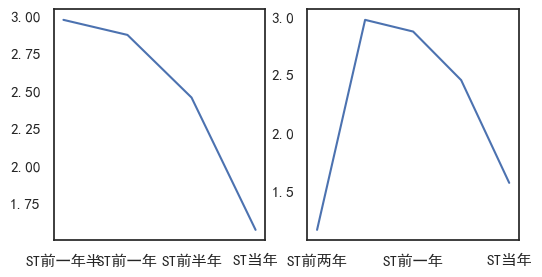
\includegraphics[width=0.8\linewidth]{img/st.png}
        \caption{一年半内持续走低,两年全量不明显}
    \end{figure}
\end{frame}

\begin{frame}
    \frametitle{预警线的设置}
    \only<1>{
        作者还做了频率统计,发现违约距离越小,ST的频率就越高,与KMV模型一致,因而作者提出可以设置信贷风险预警线:$DD=2$为二级预警线,而$DD=1$为一级预警线。
    }
    低于二级预警线有47\%的概率被ST,而低于一级预警线有81\%的概率被ST。2011年上半年有32.67\%的中小企业违约距离低于二级警戒线。
    \only<2>{复现结果显示并非如此,后验视角看也没有$47\%\times 67\% = 31.49\%$的样本内企业被ST。}
    \only<1>{
        \begin{figure}[H]
            \begin{minipage}{0.48\linewidth}
                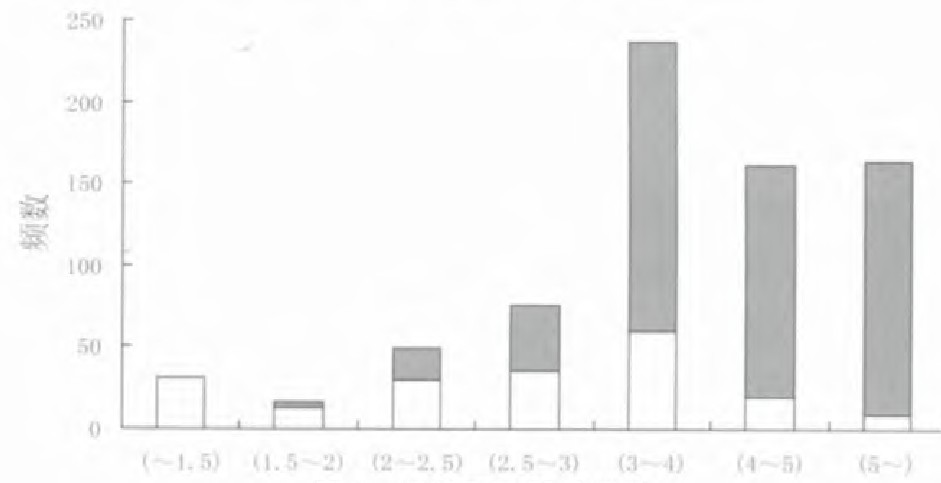
\includegraphics[width=\linewidth]{img/fig2.jpeg}
            \end{minipage}
            \begin{minipage}{0.48\linewidth}
                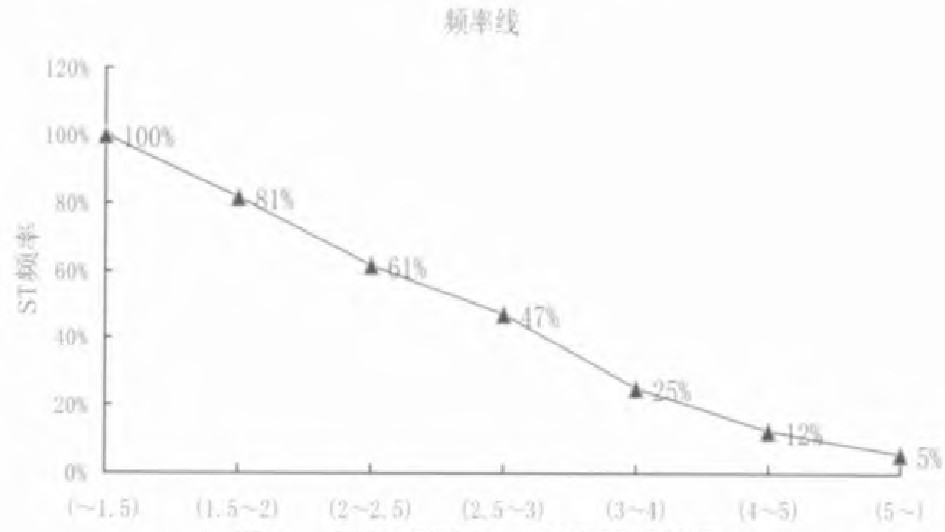
\includegraphics[width=\linewidth]{img/fig3.jpeg}
            \end{minipage}
            \caption{作者ST频数(左)与频率(右)分布图,横轴为$DD$}\label{fig:origin23}
        \end{figure}
    }
    \only<2>{
        \begin{figure}[H]
            \begin{minipage}{0.48\linewidth}
                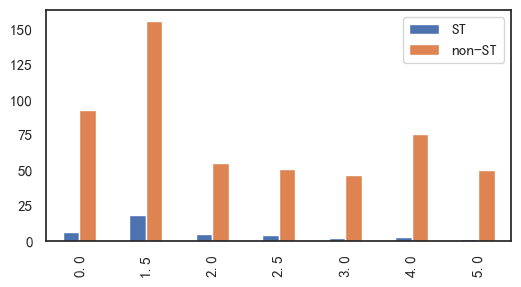
\includegraphics[width=\linewidth]{img/fig2_.png}
            \end{minipage}
            \begin{minipage}{0.48\linewidth}
                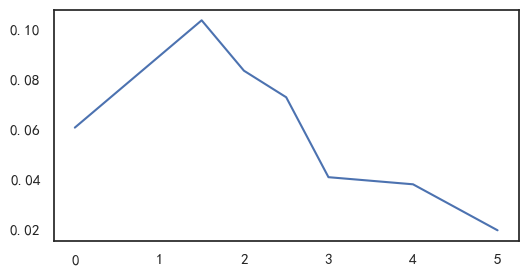
\includegraphics[width=\linewidth]{img/fig3_.png}
            \end{minipage}
            \caption{复现ST频数(左)与频率(右)分布图,横轴为$DD$}\label{fig:23}
        \end{figure}
    }
\end{frame}

\begin{frame}
    \frametitle{一类错误和II类错误的误判率}

    作者设定违约距离的临界值为$0.5\times \bar{DD}_t+0.5\times 3$,低于该临界值则预测公司违约。考虑到误差,作者在判断I类错误时将阈值上调0.3,而判断II类错误时阈值下调0.3

    \begin{columns}
        \column{0.48\linewidth}
        \begin{figure}[H]
            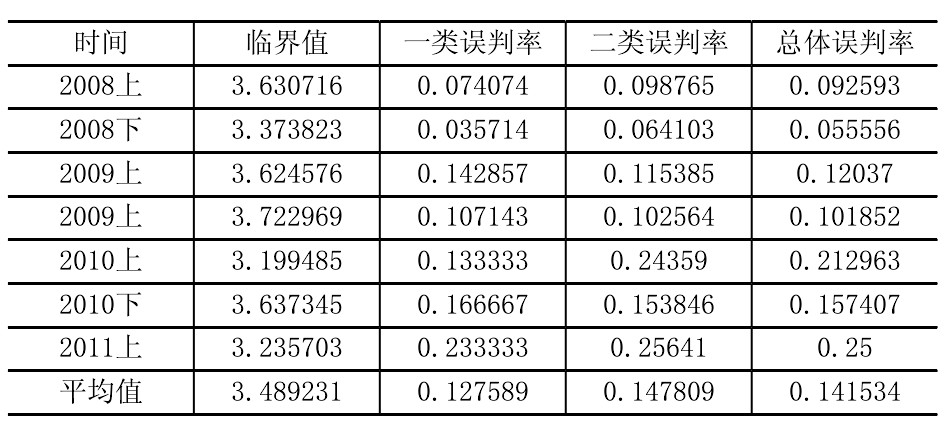
\includegraphics[width=\linewidth]{img/tab1.jpeg}
            \caption{作者的I/II类错误误判率}
        \end{figure}
        \column{0.48\linewidth}
        \begin{table}[H]
            \centering
            \begin{tabular}{lrr}
\toprule
{} &     $\alpha$ &      $\beta$ \\
\midrule
2008-06-30 &  0.000000 &  0.800000 \\
2008-12-31 &  0.000000 &  0.723684 \\
2009-06-30 &  0.200000 &  0.631579 \\
2009-12-31 &  0.000000 &  0.539474 \\
2010-06-30 &  0.333333 &  0.560000 \\
2010-12-31 &  0.333333 &  0.386667 \\
2011-06-30 &  0.666667 &  0.506667 \\
\bottomrule
\end{tabular}

            \caption{复现的I/II类错误误判率}
        \end{table}
    \end{columns}
\end{frame}


\subsection{反思与尝试}
\begin{frame}
    \frametitle{ROA是否是更好的指标}
    作者参考\citet{夏红芳2007基于}采用ROA作为企业价值的预期增长率。但 ROA本身是一个滞后性指标,只有企业在公布财报后才能更新。已有的研究更多是以无风险利率作为企业价值的预期增长率,更能满足BSM公式的无套利假设。
    \begin{figure}
        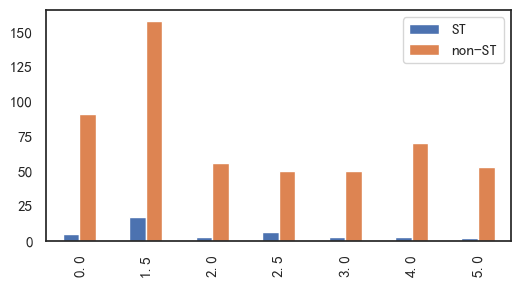
\includegraphics[width=0.8\linewidth]{fig/output.png}
        \caption{采用无风险利率结果与采用ROA基本一致}
    \end{figure}
\end{frame}


\section{心得与感悟}

\begin{frame}
    \frametitle{经验与模型}
    经验与模型哪个重要正如剑宗与气宗之争,需要结合经验与模型来对中国特色的信贷市场进行估值和分析,同时强调基本面与市场面结合交叉检验的风险分析框架。
    \begin{figure}
        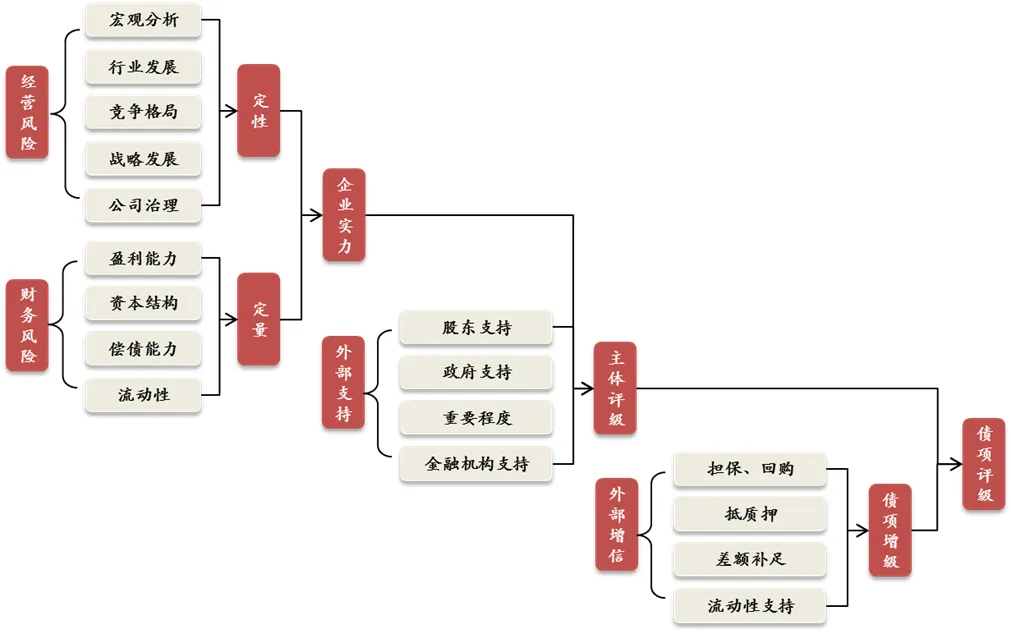
\includegraphics[width=0.8\linewidth]{fig/信用研究框架.png}
        \caption{典型的信用研究框架}
    \end{figure}
\end{frame}

\begin{frame}
    \frametitle{可能的改进方向}
    \begin{enumerate}
        \item 对信贷风险进一步落实。尽管信贷数据主要位于各国有大行手中,公开市场债券违约数据已经相对充足。可以延展到更多样本的时间序列上来观察股价波动、事件冲击(评级调整、信用事件)、财报公布等对公司违约距离的影响。
        \item 违约距离与个券收益率走势的交叉检验。可以对发行人所发行的所有债券根据其期限、余额,估值等指标构建一个加权债券指数作为其债券市场走势,与股价、违约距离三者进行交叉检验,来判断同一公司不同资产价格变动的共同趋势与差异。
        \item 增添行业补偿系数进行行业调整。KMV模型归根结底是根据资产价格是否击穿权益安全垫来判断违约风险,而不同行业负债结构差别很大,不能一概而论。运用广泛的行业打分体系也是分行业来进行财务横向比较,跨行业比较较易失真,所以当样本公司进一步增多后,应当增添行业对KMV模型的修正。
    \end{enumerate}
\end{frame}

\begin{frame}
    \frametitle{波动率对违约的影响}
    随着公开市场债券打破刚兑、资管理财产品净值化,以及宏观环境与政策冲击,后疫情时代波动率显著上升,中资高收益债走入了至暗时刻,大量的企业债券违约,大量的贷款成为坏账,甚至对中国宏观经济造成了一定的影响。“前事不忘。后事之师”,KMV模型为我们提供了一些思路,让我们思考资产的波动对企业信贷风险的影响。
    \begin{figure}
        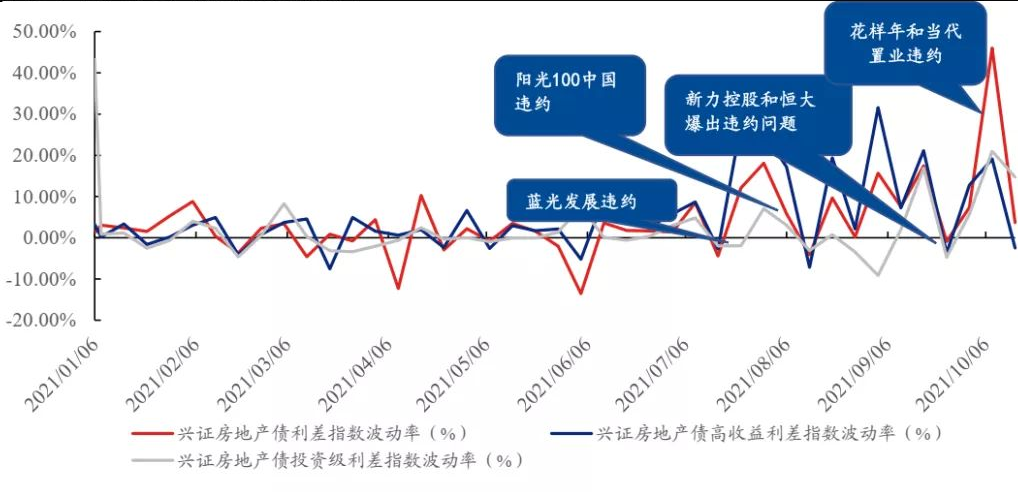
\includegraphics[width=0.8\linewidth, trim=0 20 0 0]{fig/波动率.jpeg}
        \caption{波动率}
    \end{figure}
\end{frame}

\nocite{*}
\appendix
\begin{frame}[allowframebreaks]{参考文献}
    \nocite{*}
    \tiny{\printbibliography[heading=bibliography,title=参考文献]}
\end{frame}
\end{document}
